The speech recogniser developed in this thesis is based on an end-to-end discriminative deep recurrent neural network.  Two models were developed.  The first model, a \acrlong{gru} \acrlong{rnn}  (\acrshort{gru}-\acrshort{rnn}), was used to develop a character-based \acrfull{LM}.  The second model is a \acrfull{birnn} is an end-to-end speech model capable of generating word sequences based on learned character sequence outputs.  This chapter describes the transition from generative speech models to these discriminative end-to-end recurrent neural network models.  Low speech recognition strategies are also discussed and the contribution to knowledge gained by using character-based discrimination as well as introducing deep scattering features to the bi-RNN speech model is brought to light.

\section{Speech Recognition Overview}\label{Ch_2_SROverview}
Computer speech recognition takes raw audio speech and converts it into a sequence of symbols.  This can be considered as an analog to digital conversion as a continuous signal becomes discretised.  The way this conversion is done is by breaking up the audio sequence into very small packets referred to as frames and developing discriminating parameters or features for each frame. Then, using the vector of features as input to the speech recogniser.  

A statistical formulation \citep{young2002htk} for the speech recogniser follows given that each discretised output word in the audio speech signal is represented as a vector sequence of frame observations defined in the set $\mathbf{O}$ such that 
\begin{equation}\mathbf{O}=\mathbf{o}_1,\mathbf{o}_2,\dots,\mathbf{o}_T.
\label{eqn_1_1_sr_inputs}
\end{equation}

Equation \ref{eqn_1_1_sr_inputs} says that, at each discrete time $t$, we have an observation $\mathbf{o}_t$, which is, in itself is a vector in $\mathbb{R}^D$.  From the conditional probability, it can be formulated that certain word sequences from a finite dictionary are most probable given a sequence of observations. That is:
\begin{equation}arg\max_t\{P(w_i|\mathbf{O})\}
\label{eqn_2_2_srgen}
\end{equation}

Section~\ref{sec_c2_asr_challenges} outline some challenges of  speech recognition which result in the  analysis of $P(w_i|\mathbf{O})$ being no trivial task.  The divide and conquer strategy therefore employed uses Bayes formulation to simplify the problem.  Accordingly, the argument that maximises the probability of an audio sequence given a particular word multiplied by the prior probability of that word is equivalent to the original posterior probability required to solve the original speech recognition problem. This is summarised by the following equation
\begin{equation}P(w_i|\mathbf{O})=\frac{P(\mathbf{O}|w_i)P(w_i)}{P(\mathbf{O})}
\label{eqn_2_3_bayes_sr}
\end{equation}

According to Bayes’ rule, the posterior probability is obtained by multiplying a certain likelihood probability by a prior probability.  The likelihood in this case, $P(\mathbf{O}|w_i)$, is obtained from a Hidden Markov Model (HMM) parametric model such that rather than estimating the observation densities in the likelihood probability, these are obtained by estimating the parameters of the HMM model.  The HMM model explained in the next section gives a statistical representation of the latent variables of speech at a mostly acoustic level.

The second parameter in the speech model, interpreted from Bayes' formula, is the prior probability of a given word.  This aspect of the model is the language model which is reviewed in section \ref{sec_lrlm}.

\subsection{HMM-based Generative speech model}
A HMM represents a finite state machine where a process transits a sequence of states from a set of fixed states \citep{gales2008application, young2002htk}. The overall sequence of transitions will have a start state, an end state and a finite number of intermediate states all within the set of finite states.  Each state transition emits an output observation that represents the current internal state of the system.

\begin{figure}
\centering
  % Requires \usepackage{graphicx}
  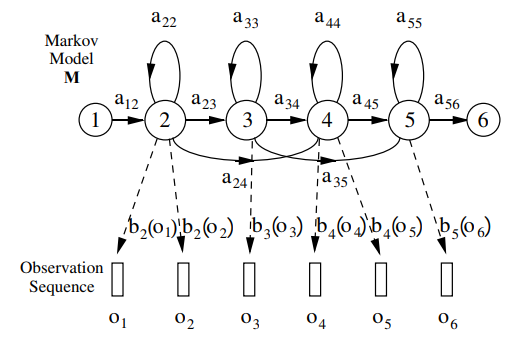
\includegraphics[width=9cm]{thesis/images/hmm}\\
  \caption{HMM Generative Model}\cite{young2002htk}\label{fig_2_1_hmm}
\end{figure}

In an HMM represented in Figure \ref{fig_2_1_hmm} there are two important probabilities.  The first is the state transition probability given by $a_{ij}$ this is the probability to move from state $i$ to state $j$.  The second probability $b_j$ is the probability that an output observation is emitted when in a particular state.

Where $\mathbf{O}$, are the output observations and $M$ is the HMM.  Given that $X$ represents the sequence of states transitioned by a process, a HMM defines the joint probability of $X$ and the output probabilities given the HMM in the following representation:
\begin{equation}P(\mathbf{O}|M)=\sum_Xa_{x(0)x(1)}\prod_{t=1}^Tb_{x(t)}(\mathbf{o}_t)a_{x(t)x(t+1)}
\label{eqn_2_4_hmm}
\end{equation}

Generally speaking, the HMM formulation presents 3 distinct challenges.  The first is the likelihood of a sequence of observations given in equation \ref{eqn_2_4_hmm} above.  The next two,  described later, is the inference and the learning problem.  While the inference problem determines the sequence of steps given the emission probabilities, the learning problem determines the HMM parameters, that is the initial transition and emission probabilities of the HMM model.

For the case of the inference problem, the sequence of states can be obtained by determining the sequence of states that maximises the probability of the output sequences.

\subsection{Challenges of Speech Recognition}\label{sec_c2_asr_challenges}
The realised symbol is assumed to have a one to one mapping with the segmented raw audio speech. However, the difficulty in computer speech recognition is the fact that there is a significant amount of variation in speech that would make it practically intractable to establish a direct mapping from segmented raw speech audio to a sequence of static symbols. The phenomena known as co articulation has it that there are several different symbols having a mapping to a single waveform of speech in addition to several other varying factors including the speaker mood, gender, age, the medium of speech transduction, the room acoustics, et cetera.

Another challenge faced by automated speech recognisers is the fact that the boundaries of the words are not apparent from the raw speech waveform. A third problem that immediately arises from the second is the fact that the words from the speech may not strictly follow the words in the selected vocabulary database.  Such occurrence in speech recognition research is referred to as \acrfull{oov} terms.  It is reasonable to approach these challenges using a divide and conquer strategy.  In this case, the first step would be to make provision for word boundaries.  This first step in speech recognition is referred to as the isolated word recognition case \citep{young2002htk}.

\subsection{Challenges of low speech recognition}
Speech recognition for low resource languages poses another distinct set of challenges.  In chapter one, low resource languages were described to be languages lacking in resources required for adequate Machine Learning of models needed for generative speech models.  These resources are described basically as a text corpus for language modelling, a phonetic dictionary and transcribed audio speech for acoustic modelling. Figure \ref{fig_2_2_asr_pipeline}, illustrates how resources required for speech recognition are utilised.  It is observed that in addition to the three resources identified other processes are required for the speech decoder to function normally.  For example, aligned speech would also need to be segmented into speech utterances to ensure that the computer resources are used conservatively.

In terms of data collection processing \cite{besacier2014automatic} enumerate the  challenges for developing low resource ASR systems to include the fact that phonologies (or language sound systems) differ across languages, word segmentation problems, fuzzy grammatical structures, unwritten languages, lack of native speakers having technical skills and the multidisciplinary nature of ASR constitute impedance to ASR system building.

\begin{figure}
\centering
  % Requires \usepackage{graphicx}
  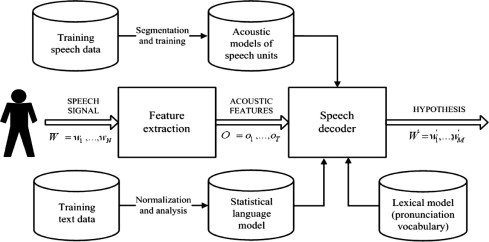
\includegraphics[width=10cm]{thesis/images/asr_pipeline}\\
  \caption{Automatic Speech Recognition Pipeline} \cite{besacier2014automatic}\label{fig_2_2_asr_pipeline}
\end{figure}

\section{Low Resource Speech Recognition}
In this system building speech recognition research, the focus was on the development of a language model and an end-to-end speech model comparable in performance to state of the art speech recognition system consisting of an acoustic model and a language model.  Low resource language and acoustic modelling are now reviewed keeping in mind that little work has been done on low-resource end-to-end speech modelling when compared to general end-to-end speech modelling and general speech recognition as a whole.  

From an engineering perspective, a practical means of achieving low resource speech modelling from a language rich in resources is through various strategies of the Machine Learning sub-field of transfer learning.  

Transfer learning takes the inner representation of knowledge derived from training algorithm used from one domain and applying this knowledge in a similar domain having different set of system parameters\citep{ramachandran2016unsupervised}. Early work of this nature for speech recognition is demonstrated in \citep{vu2013multilingual} where multi-layer perceptrons were used to train multiple languages rich in linguistic resources. In a later section entitled “speech recognition on a budget”, a transfer learning mechanism involving deep neural networks from \citep{kunze2017transfer} is described.

\subsection{Low Resource language modelling} \label{sec_lrlm}

General language modelling is reviewed and then Low resource language modelling is discussed in this section.  In section \ref{Ch_2_SROverview}, recall from equation \ref{eqn_2_3_bayes_sr}, the general speech model influenced by Bayes' theorem.
\begin{equation}P(w_i|\mathbf{O})=\frac{P(\mathbf{O}|w_i)P(w_i)}{P(\mathbf{O})}
\label{eqn_2_5_bayes_sr}
\end{equation}

The speech recognition model is a product of an acoustic model (likelihood probability),$P(\mathbf{O}|w_i)$ and the language model (prior probability),$P(w_i)$.  The development of  language models for speech recognition is discussed in \cite{juang2000automatic} and \cite{1996YoungA}.  

Language modelling formulate rules that predict linguistic events and can be modelled in terms of discrete density $P(W)$, where  $W=(w_1, w_2,..., w_L)$ is a word sequence. The density function $P(W)$ assigns a probability to a particular word sequence $W$.  This value determines how likely the word is to appear in an utterance. A sentence with words appearing in a grammatically correct manner is more likely to be spoken than a sentence with words mixed up in an ungrammatical manner, and, therefore, is assigned a higher probability. The order of words therefore reflect the language structure, rules, and conventions in a probabilistic way. Statistical language modeling therefore, is an estimate for $P(W)$ from a given set of sentences, or corpus.

The prior probability of a word sequence $\mathbf{w}=w_1,\dots,w_k$ required in equation (2.2) is given by:
\begin{equation}P(\mathbf{w})=\prod_{k=1}^KP(w_k|w_{k-1},\dots,w_1)
\label{eqn_c2_lm01}
\end{equation}

The N-gram model is formed by the conditioning of the word history in equation \ref{eqn_c2_lm01}.  This therefore becomes:
\begin{equation}P(\mathbf{w})=\prod_{k=1}^KP(w_k|w_{k-1},w_{k-2},\dots,w_{k-N+1})
\label{eqn_c2_lm02}
\end{equation}

N is typically in the range of 2-4.

N-gram probabilities are estimated from training corpus by counting N-gram occurrences.  This is plugged into maximum likelihood (ML) parameter estimate. For example, Given that N=3 then the probability that three words occurred is assuming $C(w_{k-2}w_{k-1}w_k)$ is the number of occurrences of the three words $C(w_{k-2}w_{k-1})$ is the count for $w_{k-2}w_{k-1}w_k$ then
\begin{equation}
P(w_k|w_{k-1},w_{k-2})\approx\frac{C(w_{k-2}w_{k-1}w_k)}{C(w_{k-2}w_{k-1})}
\label{eqn_c2_lm03}
\end{equation}

The major problem with maximum likelihood estimation scheme is data sparsity. This can be tackled by a combination of smoothing techniques involving discounting and backing-off.  The alternative approach to robust language modelling is the so-called class based models \citep{Brown1992class,Kuhn1990cache} in which data sparsity is not so much an issue.  Given that for every word $w_k$, there is a corresponding class $c_k$, then,
\begin{equation}
P(\mathbf{w})\prod_{k=1}^KP(w_k|c_k)p(c_k|c_{k-1},\dots,c_{k-N+1})
\label{eqn_c2_lm04}
\end{equation}

In 2003,  \cite{bengio2003neural} proposed a language model based on neural Multi-Layer Perceptrons (MLPs). These MLP language models resort to a distributed representation of all the words in the vocabulary such that the probability function of the word sequences is expressed in terms of these word-level vector representations. The performance of the MLP-based language models was found to be, in cases for models with large parameters,  better than the traditional n-gram models.

Improvements over the MLPs still using neural networks over the next decade include works of \cite{mikolov2011empirical,sutskever2014sequence,luong2013better}, involved the utilisation of deep neural networks for estimating word probabilities in a language model.  While a Multi-Layer Perceptron consists of a single hidden layer, in addition to the input and output layers, a deep network, in addition to having several hidden layers, is characterised by complex structures that render the architecture beyond the basic feed forward nature. Particularly, for Recurrent Neural Network (RNN) architectures, we also have some feedback neurons in addition to the forward neurons where data flows in the reverse direction, from output to input. 

Furthermore, the probability distributions in these deep neural networks were either based upon word or sub-word models, this time having representations which also conveyed some level of syntactic or morphological weights to aid in establishing word relationships.  These learned weights are referred to as token or unit embedding \citep{pennington-etal-2014-glove}.

For the neural network implementations so far seen, a large amount of data is required due to the nature of words to have large vocabularies, even for medium-scale speech recognition applications.   \cite{kim2016character} on the other hand took a different approach to language modelling taking advantage of the long-term sequence memory of long-short-term memory cell recurrent neural network (LSTM-RNN) to model a language based on characters rather than on words.  This greatly reduced the number of parameters involved and therefore the complexity of implementation.  This method is forms the basis of the Wakirike language model implementation in this work due to the low resource constraints gains made when using a character-level language model.

Other low resource language modelling strategies employed for the purpose of speech recognition was demonstrated by \cite{xu2013cross}.  The language model developed in that work was based on phrase-level linguistic mapping from a high resource language to a low resource language using a probabilistic model implemented using a \acrfull{wfst}.  This method uses \acrshort{wfst} rather than a neural network due to scarcity of training data required to develop a neural network. However, it did not gain from the high non linearity ability of a neural network model to discover hidden patterns in data, being a shallower Machine Learning architecture.

The language model implemented in this thesis report uses a character-based Neural network language model that employs a recurrent neural network similar to that of \cite{kim2016character}, however based on \acrfull{gru} \acrshort{rnns} \citep{cho2014learning}, for the Okrika language which is a low resource language, bearing in mind that the character level network will reduce the number of parameters required for training, just enough to develop a working language model for the purpose of speech recognition. 

\subsection{Low Resource Acoustic and speech modelling}

Two transfer learning techniques for acoustic modelling investigated by \cite{povey2011subspace} and \cite{ghoshal2013multilingual} respectively include the \acrfull{sgmm} and the use of pretrained hidden layers of a deep neural network trained multilingually as a means to initialise weights for an unknown language.  This second method of low resource modelling has been informally referred to as the swap-hat method.

Recall that one of the challenges associated with new languages is that phonetic systems differ from one language to another.  Transfer learning approaches attempt however to recover patterns common to seemingly disparate systems and model these patterns.  

The physiologic speech production mechanism is based on the premise that sounds are produced by approximate movements and positions of articulators that comprise the human speech production system and that this mechanism is common to all humans.  It is possible to model dynamic movement from between various phones as tied state mixture of Gaussians. These dynamic states modelled using \acrfull{gmm} are also called senones. \cite{povey2011subspace} postulated a method to factorize these Gaussian mixtures into a globally shared set of parameters that are non-dependent individual HMM states.  These factorisations model senones that are not represented in original data and thought to be a representation of the overall acoustic space.  While preserving individual HMM states, the decoupling of the shared space and its reuse makes SGMMs a viable candidate for transfer learning of acoustic models for new languages.

The transfer learning procedure proposed in \cite{ghoshal2013multilingual} employed the use of \acrlong{dnns}, in particular \acrfull{dbn}s \citep{bengio2007greedy}.  \acrlong{dbn}s are pretrained, layer-wise  stacked \acrlong{rbn}s (RBMs)\citep{smolensky1986information}.  The output of this network trained on senones correspond to HMM context dependent states.  However, by decoupling hidden layers from outer and output layers and fine-tuned to a new language, the network is shown to be insensitive to the choice of languages analogous to global parameters of SGMMs. The 7-layer, 2000 neuron per layer network used did not utilise a bottleneck layer corresponding to triphone states trained on MFCC features \citep{grezl2008optimizing}.

\section{Groundwork for low resource end-to-end speech modelling}
The underpinning notion of this work is firstly a departure from the extra processing required for  bottom-to-top that comes as a byproduct of the generative process sponsored by the HMM-based speech models. This has an advantage of simplifying the speech pipeline from acoustic, language and phonetic model to just a speech model that approximates the same process.  Secondly, the model developed seeks to overcome the data intensity barrier and was seen to achieve measurable results for GRU RNN language models.  Therefore adopting the same character-based strategy, this research performed experiments using the character-based bi-directional recurrent neural networks (BiRNN).  However, BiRNNs researchers have found them like other deep learning algorithms, too be quite data intensive\cite{hannun2014deep}.  The next paragraphs introduce Deep-speech BiRNNs and the two strategies for tackling the data intensity drawback as related with low resource speech recognition.

\subsection{Deep speech}
Up until recently, speech recognition research has been centred on improvements of the HMM-based acoustic models.  This has included a departure from generative training of HMM to discriminative training \citep{woodland2000large} and the use of neural network precursors to initialise the HMM parameters \citep{mohamed2012acoustic}.  Although these  discriminative models brought improvements over generative models, being HMM dependent speech models they lacked the end-to-end nature.  This means that they were subject to training of acoustic, language and phonetic models.  With the introduction of the \acrfull{ctc} loss  function, \cite{graves2014towards} finally found a means to end-to-end speech recognition departing from HMM-based speech recognition. 

The architecture of the Deep-speech end-to-end speech recognition model \cite{hannun2014first} follows an end-to-end Bi-directional Recurrent Neural Network (BiRNN) and CTC loss function \citep{graves2006connectionist}.  The CTC loss function uses a modified beam search to sum over all viable sequences of the input and output sequence space alignments so as to maximise the likelihood of the output sequence characters.

\subsection{Speech Recognition on a low budget}

In this section, a recent transfer learning speech model \citep{kunze2017transfer} that has some characteristics similar to the speech model developed in this thesis is reviewed.  The end-to-end speech model described by \cite{kunze2017transfer} is based on that developed by \cite{collobert2016wav2letter} and is based on deep convolutional neural networks rather than the Bi-RNN structure proposed by this work.  In addition it uses a loss function based on the AutoSegCriterion which is claimed to work competitively with raw audio waveform without any preprocessing.  The main strategy for low resource management in their system was the freezing of some layers within the convolutional network layer.  The low resource mechanisms used in this work includes the use of a unique scattering network being used as input features for the BiRNN model.  The fascinating similarity between the end-to-end BiRNN speech model developed in this work and the transfer learning model in \cite{kunze2017transfer} is the fact that the scattering network input is equivalent to the output of a light-weight convolutional neural network \cite{hannun2014first}.  Therefore the proposed system then approximates a combination of a recurrent neural network as well as a convolution neural network without the overhead of actually training a convolutional neural network (CNN)\citep{szegedy2015going}.

Introduction of the unique scattering network is discussed in the next section.  It is worthy to note however that \cite{kunze2017transfer} uses a CNN network only while \citep{amodei2016deep} uses both RNN and CNN network.  The speech model in this thesis uses a BiRNN model and combines an RNN model with the scattering layer which represents a light-weight low resource friendly pseudo enhanced CNN backing.  What is meant by pseudo enhanced CNN backing is reserved for the next section, however, therefore, the proposed speech model in this thesis stands to gain from an enhanced but lightweight \acrshort{cnn} combined with \acrshort{rnn} learning.

\subsection{Adding a Scattering layer}

In Machine Learning, training accuracy is greatly improved through a process described as feature engineering.  In feature engineering, discriminating characteristics of the data are enhanced at the same time non-distinguishing features constituting noise are removed or attenuated to a barest minimum.  A lot of the components signal speech signal are due to noise in the environment as well as signal channel distortions such as losses due to conversion from audio signals to electrical signal in the recording system.

In Figure \ref{fig_2_2_asr_pipeline}, feature engineering is done at the feature extraction stage of the ASR pipeline. It has been shown that a common technique using \acrfull{mfcc} \citep{davis1980comparison} can represent speech in a stable fashion that approximate how the working of the human auditory speech processing and is able to filter useful components in the speech signal required for human speech hearing. Similar feature processing schemes have been developed include \acrfull{plp} \citep{hermansky1990perceptual} and \acrfull{rasta} \citep{hermansky1994rasta}. 

The scattering spectrum defines a locally translation invariant representation of a signal resistant to signal deformation over extended periods of time spanning seconds of the signal \citep{anden2014deep}. While Mel-frequency cepstral coefficients (MFCCs) are cosine transforms of Mel-frequency spectral coefficients (MFSCs), the scattering operator consists of a composite wavelet and modulus operation on input signals. 

Over a fixed time, MFSCs measure signal energy having constant Q bandwidth Mel-frequency intervals.  This procedure is susceptible to time-warping signal distortions since these information often reside in the high frequency regions discarded by Mel-frequency intervals.  As time-warping distortions is not explicit classifier objective when developing these filters, there is no way to recover such information using current techniques. 

In addition, short time windows of about 20 ms are used in these feature extraction techniques since at this resolution speech signal is mostly locally stationary.  Again, this resolution adds to the loss of dynamic speech discriminating information on signal structures that are non-stationary at this time interval. To minimize this loss Delta-MFCC and Delta-Delta-MFCCs \citep{furui1986speaker} are some of the means developed to capture dynamic audio signal characterisation over  larger time scales.

By computing multi-scale co-occurrence coefficients from a wavelet-modulus operation, \cite{anden2011multiscale} show that non-stationary attributes of a signal lost by MFSC coefficients is regained in multi scale co-occurrence coefficients. The scattering transform therefore, derives a scattering representation with an interpretation similar to MFSC-like measurements.  Together with higher-order co-occurrence coefficients, deep scattering spectrum coefficients represent audio signals similar to  models based on cascades of constant-Q filter banks and rectifiers.  In particular, second-order co-occurrence coefficients contain relevant signal information capable of discriminating dynamic information lost to the MFCC analog over several seconds and therefore a more efficient discriminant than the MFCC representation. Second-order co-occurrence coefficients calculated by cascading wavelet filter banks and rectified using modulus operations have been evaluated as equivalent to a light-weight convolutional neural networks whose output posteriors are computed at each layer instead of only at the output layer \citep{mallat2016understanding}.

The premise for this work is that low speech recognition can be achieved by having higher resolution features for discrimination as well as using an end-to-end framework to replace some of the cumbersome and time-consuming hand-engineered domain knowledge required in the standard ASR pipeline.  In addition, this research work makes contributions to the requirements for the two tracks specified in the Zero Resource challenge of 2015 \citep{versteegh2015zero}.  The first requirement is sub-word modelling satisfied by using deep scattering network and the second that of spoken term discovery criteria being satisfied by the end-to-end speech model supplemented with a language model.


\section{Chapter Summary}
Chapter \ref{ch1_intro} introduces the key terms Discriminative and Generative classification.  In this Chapter, these two different classification mechanisms are compared and contrasted as they relate to speech recognition.  The \acrfull{hmm} is considered as the key Generative algorithm used in speech recognition.  This chapter discusses the \acrshort{hmm} algorithm and outlines its limitations in speech recognition.  Other challenges associated with speech recognition and low speech recognition are discussed.  

The method taken by this research towards low resource recognition is described as well as current related research in speech recognition involving low resource discriminative strategies.  In addition, transfer learning approaches in low speech speech recognition are previewed. This chapter also outlines the addition of a scattering layer towards increasing discriminating feature tangibility for speech recognition.
